\documentclass{neu_handout}
\usepackage{url}
\usepackage{amssymb}
\usepackage{amsmath}
\usepackage{marvosym}
\usepackage{graphicx}
\usepackage[pdftex]{graphicx}
\usepackage{subfigure}
\graphicspath{ {images/} }
\everymath{\displaystyle}

% Professor/Course information
\title{A Bayseian Approach to Fake News}
\author{Emily Dutile, Shubhi Mittal, Linghan Xing}
\date{December 2017}
\course{CS5100}{Foundations of AI}

\begin{document}
\section*{1 Introduction and Background}

"Fake news" became an increasingly coined term and was almost non-existent in the general context and media providers prior to October 2016 of the Presidential Election. In late 2016, the top 20 fake news stories on Facebook were reported to outperform the top 20 real news stories, which was determined by the number of comments, reactions, and shares. As seen in figure a, it is shown the the number of real news stories did not outperform the number of fake news stories towards the end of 2016. Undoubtedly, these stories and articles our shaping and influencing the thoughts and opinions of millions of individuals and companies need to step in to help stop the spread of fake news.
\\\\
With companies such as Facebook and Google who provide ad revenue to sites that host news stories, it should be the responsibility of these tech companies to be accountable for what content is displayed. Filtering out false information in order to correctly inform and educate our society, especially when it comes to presidential elections, is an extremely important and challenging task. Companies such as Signal Media have built AI-powered media monitoring in order to help this problem after they had discovered 'fake news' as being a headline in 27,000 articles over the course of the year (see figure b).

\begin{figure}[h]
\centering
\subfigure[BuzzFeed News]
{
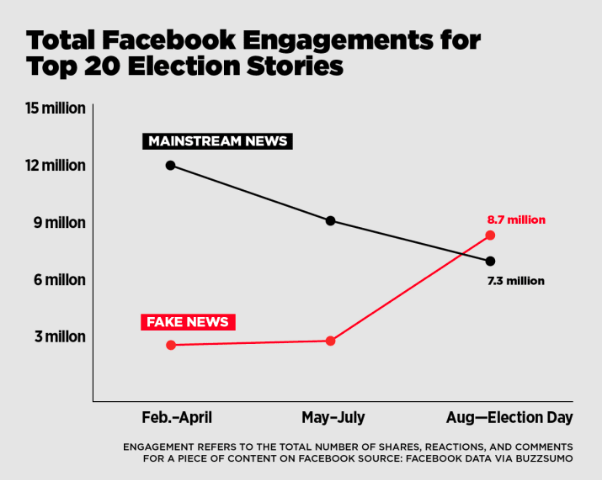
\includegraphics[width=0.3\linewidth]{buzzfeed}
}
\subfigure[]
{
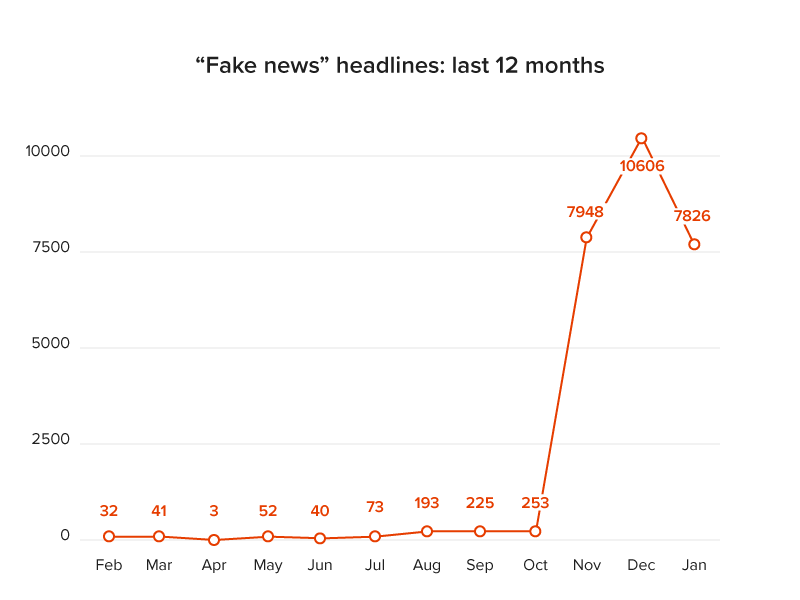
\includegraphics[width=0.3\linewidth]{fakenews}
}
\end{figure}

Fake news posts have exploited the feeds of Facebook users' which could deeply impact the options of our society if we loose our ability over time to decipher fake news from real news. Due to this problem, the data science community has looked to respond to this problem through a Kaggle competition called the Fake News Challenge \footnote{\url{http://www.fakenewschallenge.org}}. Determining real news from fake news is an extremely challenging task within the machine learning and natural language processing community. Creating models that accurately filter out fake news without removing real news sources is a very complicated task. In our approach to tackle this problem, we wanted to combat fake news by implementing a bayesian model that can differentiate fake news from real news. Expanding on this original approach, we have implemented several supervised machine learning based algorithms in order to compare text classifiers on fake news recognition. 


\subsection*{1.1 The Data}
What makes this challenge interesting and hard is around the very definition of fake news. Since we did not want to be bogged down by deciphering, scraping the web, and labeling fake news vs. real news, we found a dataset that contains almost 11,000 articles that are tagged as either real or fake news \footnote{\url{https://github.com/GeorgeMcIntire/fake_real_news_dataset}}. 


\subsection*{1.2 Methods}
We performed supervised machine learning techniques such as naive bayes, multinominal bayes with count vector and TF-IDF, along with SVM and Random Tree Forest. With respect to language processing, tokenization, filtering, lemmatization, and stemming were all used for preprocessing the titles and body text of the articles in the data set. For our evaluation process, we used a confusion matrix to understand the accuracy of our models.

\subsection*{1.3 Related Work}


\section*{2 Supervised Approach}

\subsection*{2.1 Naive Bayes}

\subsection*{2.2 Multinominal Naive Bayes}

\subsubsection*{2.2.1 Count Vectorization}


\subsubsection*{2.2.2 TF-IDF}


\subsection*{2.2 SVM}


\subsection*{2.3 Random Forest}
 
 
\subsection*{2.4 Neural Network}


\section*{3 Evaluation}

\section*{4 Acknowledgments}


\begin{thebibliography}{9}

\bibitem{ai} 
Russel and Norvig. 
\textit{Artificial Intelligence: A Modern Approach, 3rd Ed.}. 

 
\bibitem{buzzfeed}  
\textit{This Analysis Shows How Viral Fake Election News Stories Outperformed Real News on Facebook}.
[\textit{BuzzFeed News, November 2016}].
\url{https://www.buzzfeed.com/craigsilverman/viral-fake-election-news-outperformed-real-news-on-facebook?utm_term=.tnpJN34BM#.yfV6V10ZX}.
 

\bibitem{Signal}  
\textit{12 Months of Fake News Headlines, Dissected with Media Monitoring}. 
 \url{https://signalmedia.co/media-monitoring-blog/fake-news-dissected-media-monitoring/}.

\end{thebibliography}


\end{document}